\documentclass{beamer}
\usepackage[utf8]{inputenc}
\usepackage{tikz}
\usepackage{xcolor}
\usepackage{pdfpages}
\usetikzlibrary{positioning}
\usetheme{metropolis}           % Use metropolis theme
\title{Dipartimento di Ingegneria dell'Informazione}
\date{\today}
\author{}
\institute{Università degli Studi di Padova}
\begin{document}
	\begin{frame}
		\maketitle
		\begin{tikzpicture}[overlay, remember picture]
		% \node[above right=1cm and .8cm of current page.south west] {
\includegraphics[width=2cm]{logo.png}};
		% \node[above =1cm of current page.south] {
\includegraphics[width=2cm]{logo.png}};
		\node[above left=1cm and .8cm of current page.south east] {
\includegraphics[width=2cm]{logo.png}};
		\end{tikzpicture}
	\end{frame}
  \section{Quanti anni devo studiare?}
  \begin{frame}{Corso di studi}
    \centering
		\begin{figure}
  		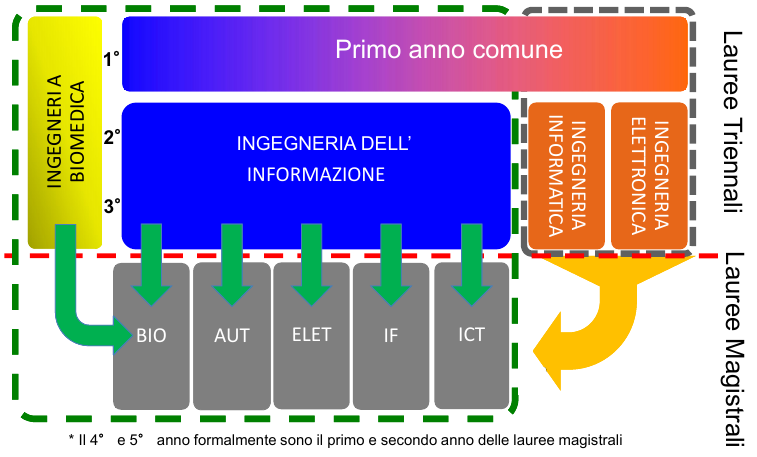
\includegraphics[width=10cm]{percorso.png}
  	\end{figure}
  \end{frame}
  \section{Come si accede?}
  \begin{frame}{Accesso programmato}
		\centering
		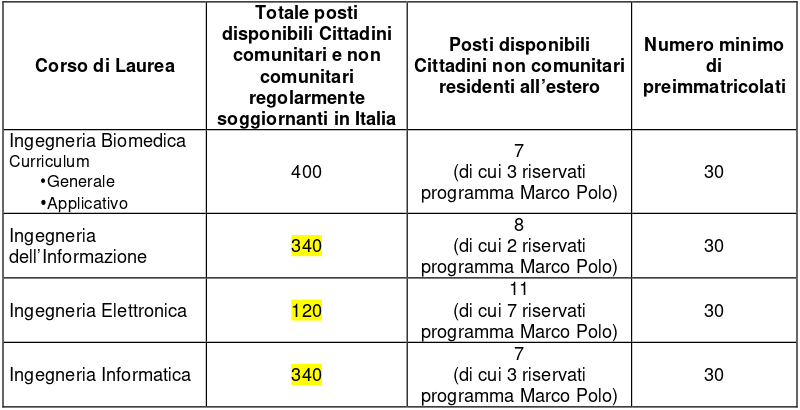
\includegraphics[width=0.6\textwidth]{posti_dei.png}

		Per un totale di 1200 posti!!\\
		Nell'A.A. 2016/2017 si sono iscritti 808 studenti in tutto

		4 sessioni d'esame, tipicamente a:\\
		Marzo, Maggio, Luglio, Agosto/Settembre

		\textbf{Pagina di riferimento:} https://www.unipd.it/avvisi-ammissione-lauree-triennali-ciclo-unico
  \end{frame}
	\section{Come faccio a laurearmi?}
	\begin{frame}{Crediti Formativi (CFU)}
		Ogni anno è necessario conseguire circa 60 crediti formativi, per un totale di \textbf{180 CFU in triennale} e \textbf{120 CFU in magistrale}.

		Dopo aver passato un esame si \textit{guadagnano} alcuni punti CFU, \textbf{in linea generale} più un esame è grosso e difficile più CFU fa \textit{guadagnare}.
	\end{frame}
	\begin{frame}{Crediti Formativi (CFU)}
		\centering
		\textbf{1 CFU $\leftrightarrow$ 25 ore di lavoro}

		\textbf{1 CFU $\leftrightarrow$ 8 ore di lezione e 17 di studio individuale}
	\end{frame}
	\section{Cosa studio a Ingegneria dell'Informazione?}
	{
		\setbeamercolor{background canvas}{bg=}
		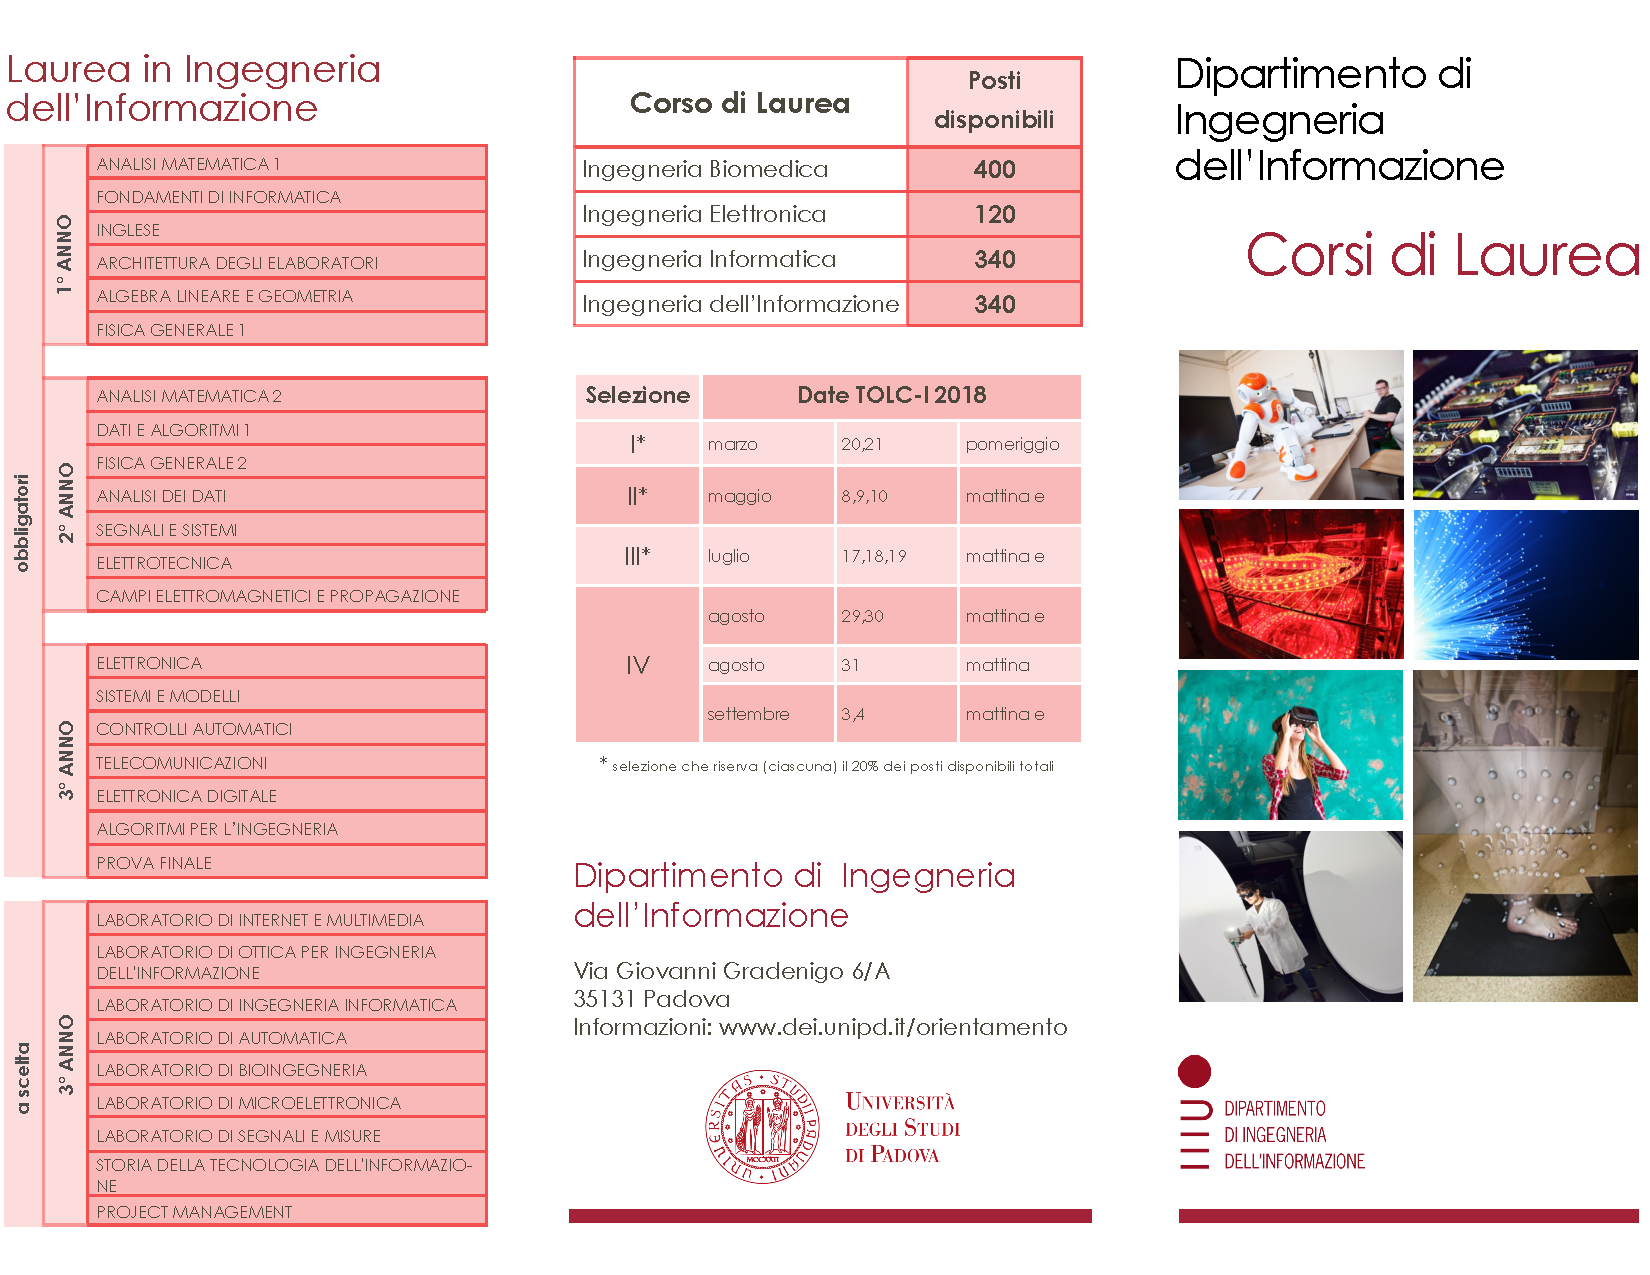
\includepdf[pages=-]{VolantinoFRONTE.pdf}
	}
		{
		\setbeamercolor{background canvas}{bg=}
		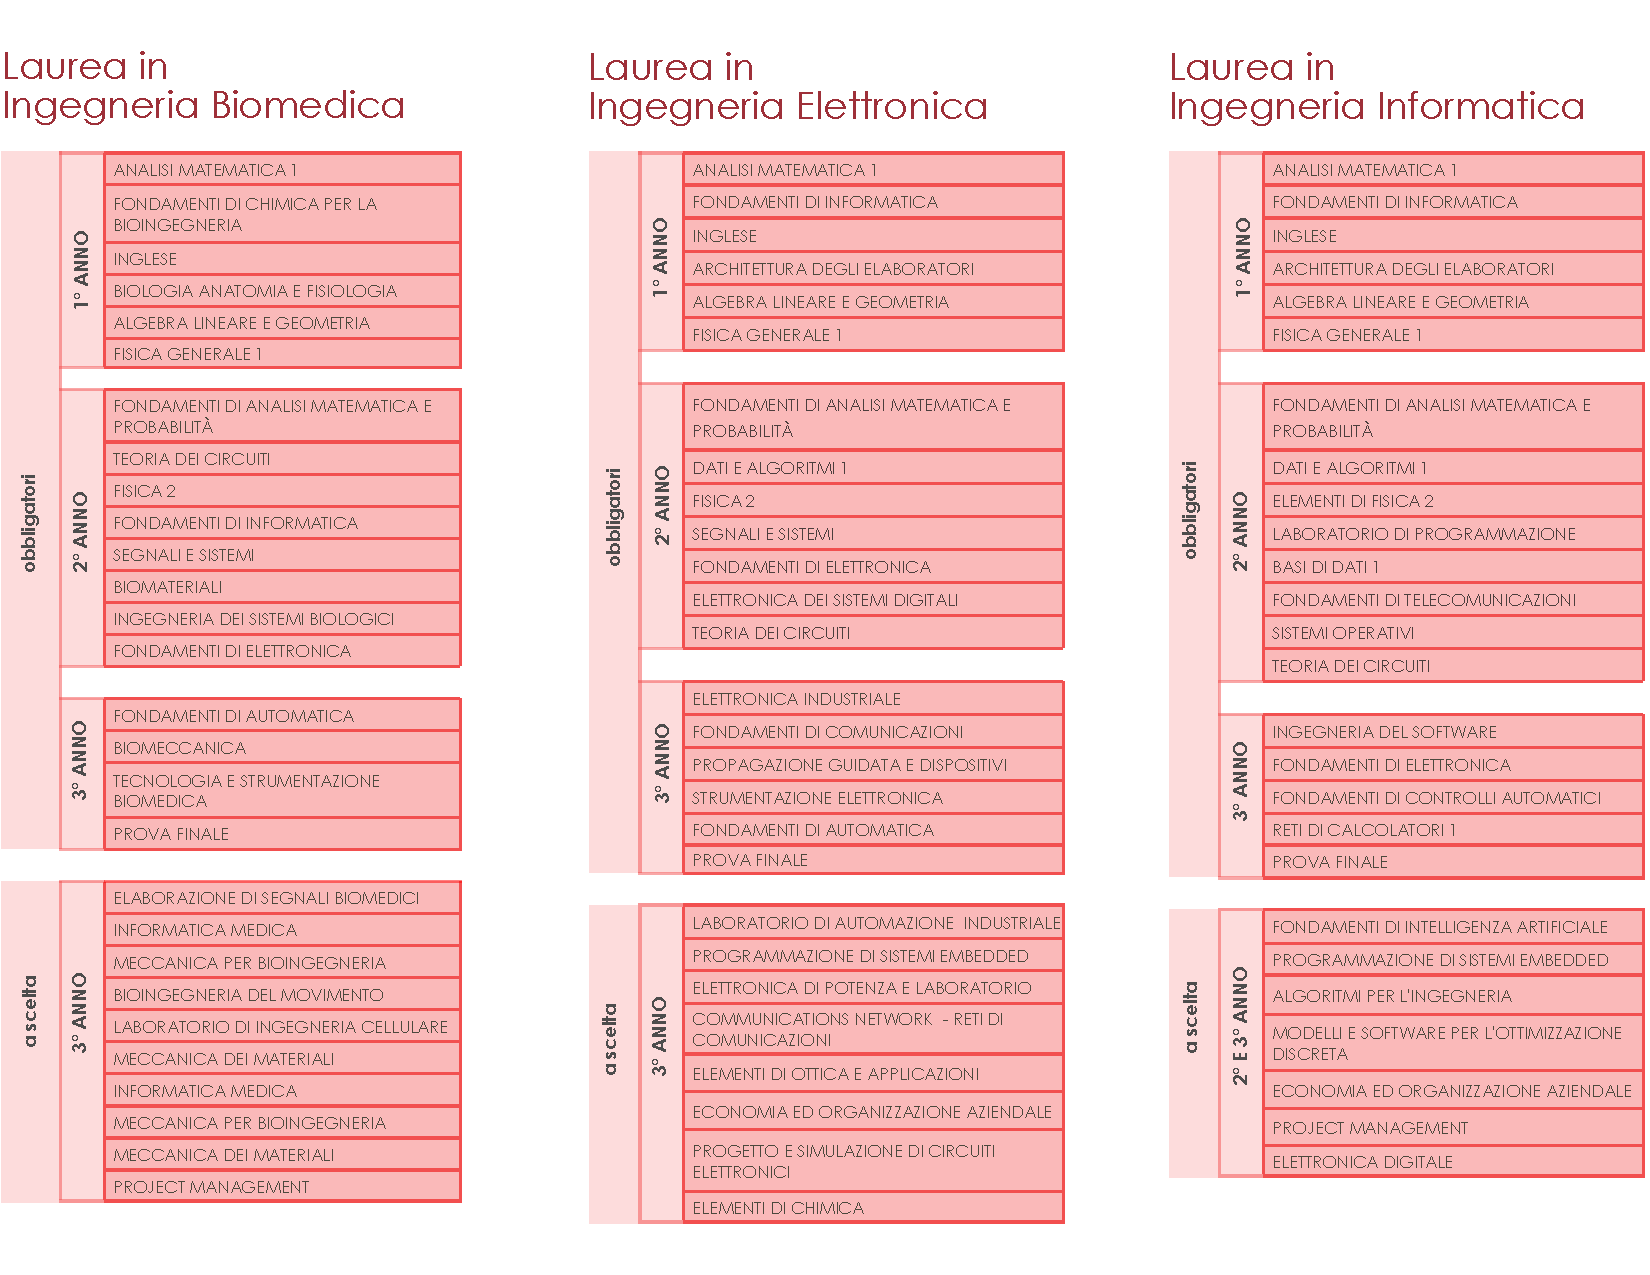
\includepdf[pages=-]{VolantinoRETRO.pdf}
	}
	\begin{frame}
		\begin{description}
			\setlength\itemsep{1em}
			\item[Laurea Triennale in Ingegneria dell'Informazione] https://didattica.unipd.it/off/2018/LT/IN/IN0513
			\item[Laurea Triennale in Ingegneria Biomedica] https://didattica.unipd.it/off/2018/LT/IN/IN2374
			\item[Laurea Triennale in Ingegneria Informatica] https://didattica.unipd.it/off/2018/LT/IN/IN0508
			\item[Laurea Triennale in Ingegneria Elettronica] https://didattica.unipd.it/off/2018/LT/IN/IN0507
		\end{description}
	\end{frame}
	\section{E dopo la triennale?}
	\begin{frame}{Lauree Magistrali}
		\textbf{
			\begin{itemize}
				\setlength\itemsep{1em}
				\item[ ] Ingegneria Informatica
				\item[ ] Ingegneria Elettronica
				\item[ ] Ingegneria dell'Automazione
				\item[ ] Bioingegneria
				\item[ ] ICT for Internet and Multimedia
				\item[ ] {\color{gray}Laurea magistrale in un'altra università italiana o all'estero!}
			\end{itemize}
		}
	\end{frame}
	\begin{frame}{LM in Ingegneria Informatica}
		\begin{columns}
			\begin{column}{0.4\textwidth}
				\centering
				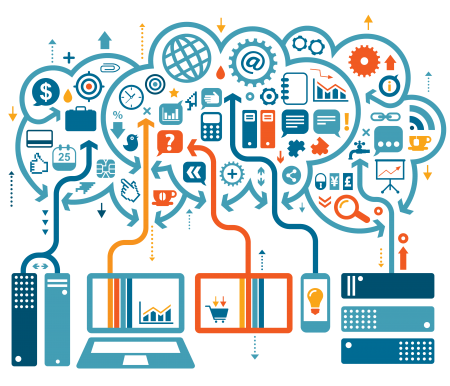
\includegraphics[width=0.6\textwidth]{big_data.png}

				Big Data

				\vspace{0.5cm}
				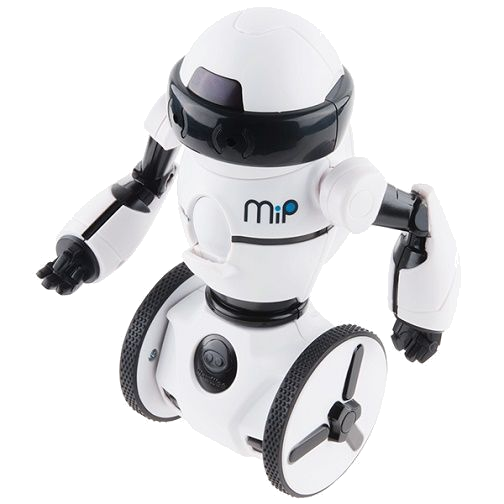
\includegraphics[width=0.6\textwidth]{robotica_inf.png}

				Robotica e Intelligenza Artificiale
			\end{column}
			\begin{column}{0.4\textwidth}
				\centering
				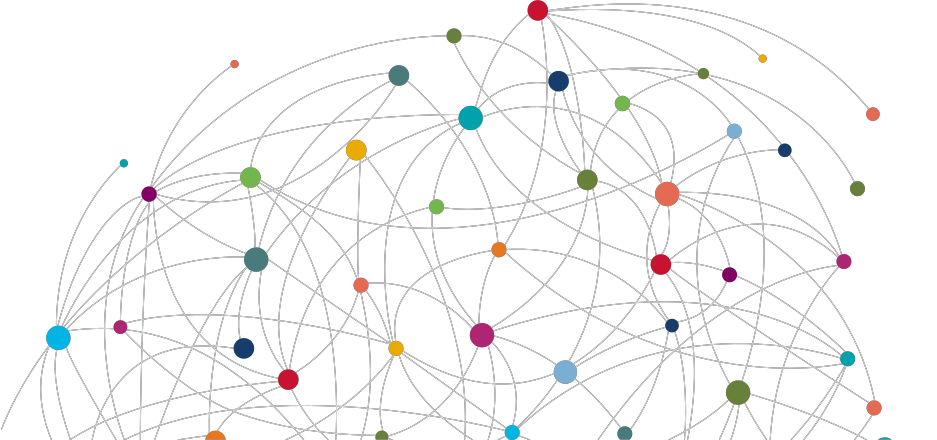
\includegraphics[width=0.8\textwidth]{network.png}

				Reti sociali, di calcolatori e IoT

				\vspace{1cm}
				
\includegraphics[width=\textwidth]{sistemi-operativi.png}

				Sistemi Operativi
			\end{column}
		\end{columns}
	\end{frame}
	\begin{frame}{LM in Ingegneria Elettronica}
		\begin{columns}
			\begin{column}{0.4\textwidth}
				\centering
				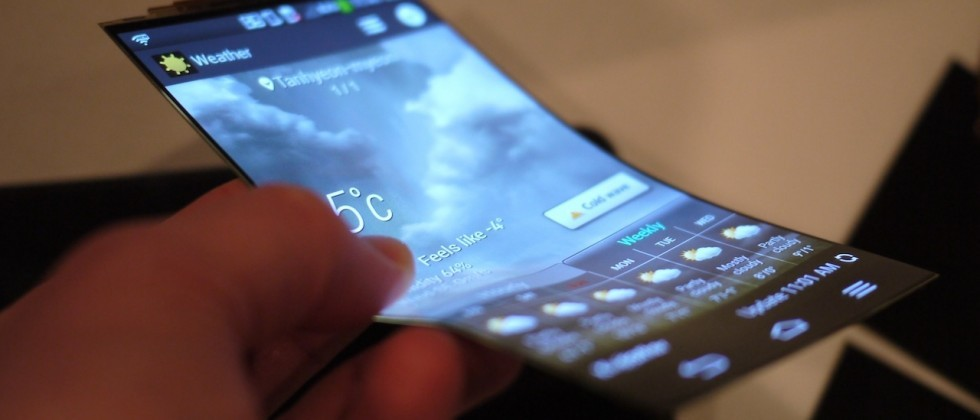
\includegraphics[width=\textwidth]{oled-lg.jpeg}

				Green Electronic

				\vspace{0.7cm}
				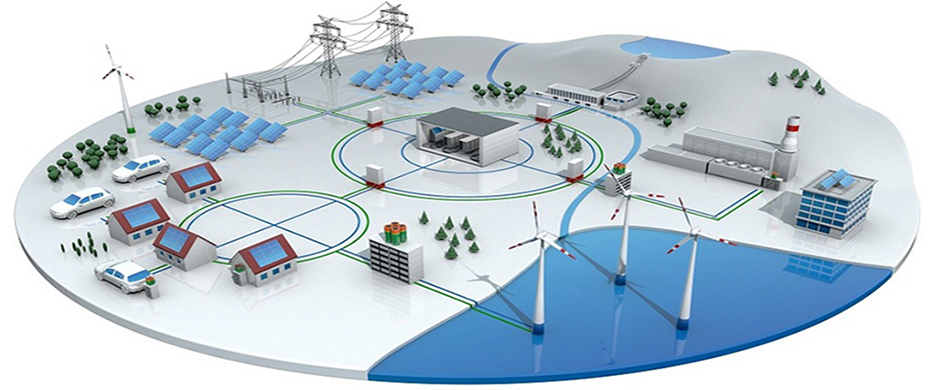
\includegraphics[width=\textwidth]{smart_grid.jpeg}

				Smart Grids e elettronica per l'energia
			\end{column}
			\begin{column}{0.4\textwidth}
				\centering
				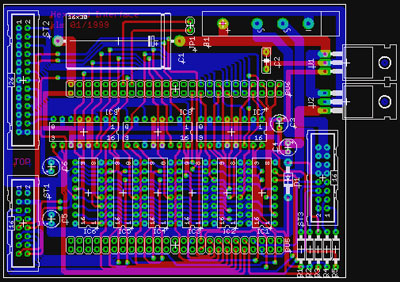
\includegraphics[width=0.8\textwidth]{prog_integr.jpeg}

				Progettazione di circuiti e sistemi integrati

				\vspace{0.3cm}
				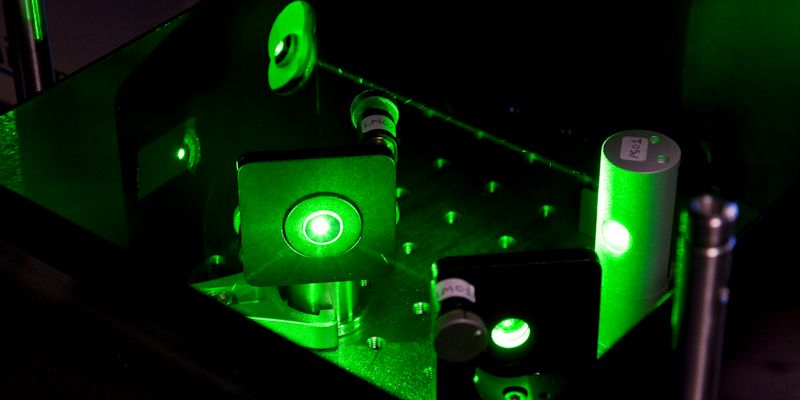
\includegraphics[width=\textwidth]{quantum_electronics.jpeg}

				Elettronica Quantistica e Optoelettronica
			\end{column}
		\end{columns}
	\end{frame}
	\begin{frame}{LM in Ingegneria dell'Automazione}
		\begin{columns}
			\begin{column}{0.4\textwidth}
				\centering
				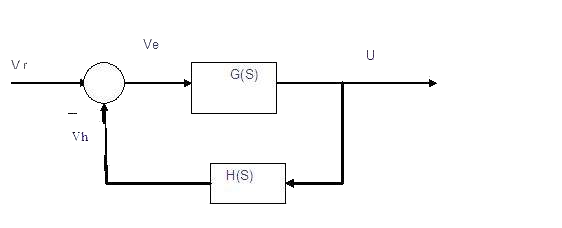
\includegraphics[width=\textwidth]{sistemi.png}

				Teoria dei Sistemi e del Controllo

				\vspace{0.5cm}
				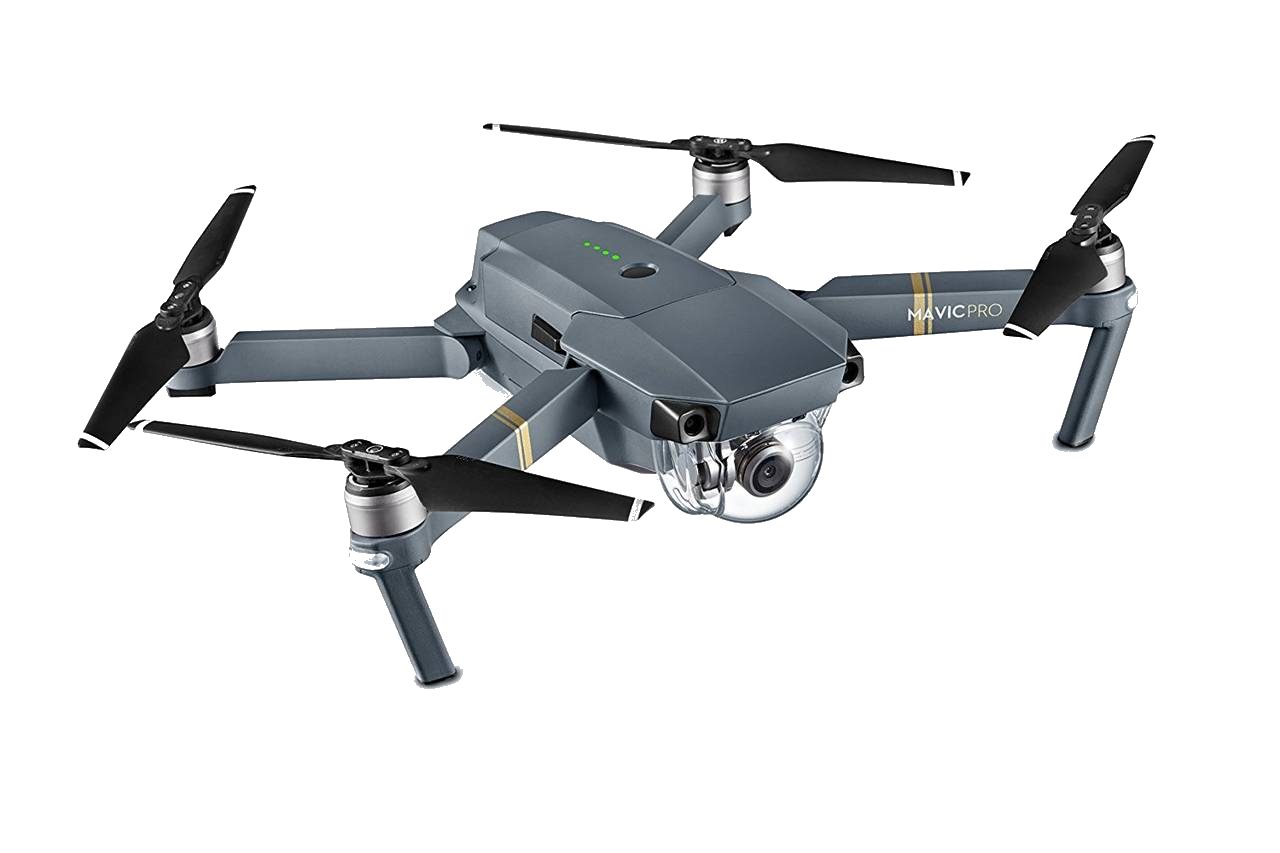
\includegraphics[width=\textwidth]{robotica_aut.png}

				Robotica e Controllo
			\end{column}
			\begin{column}{0.4\textwidth}
				\centering
				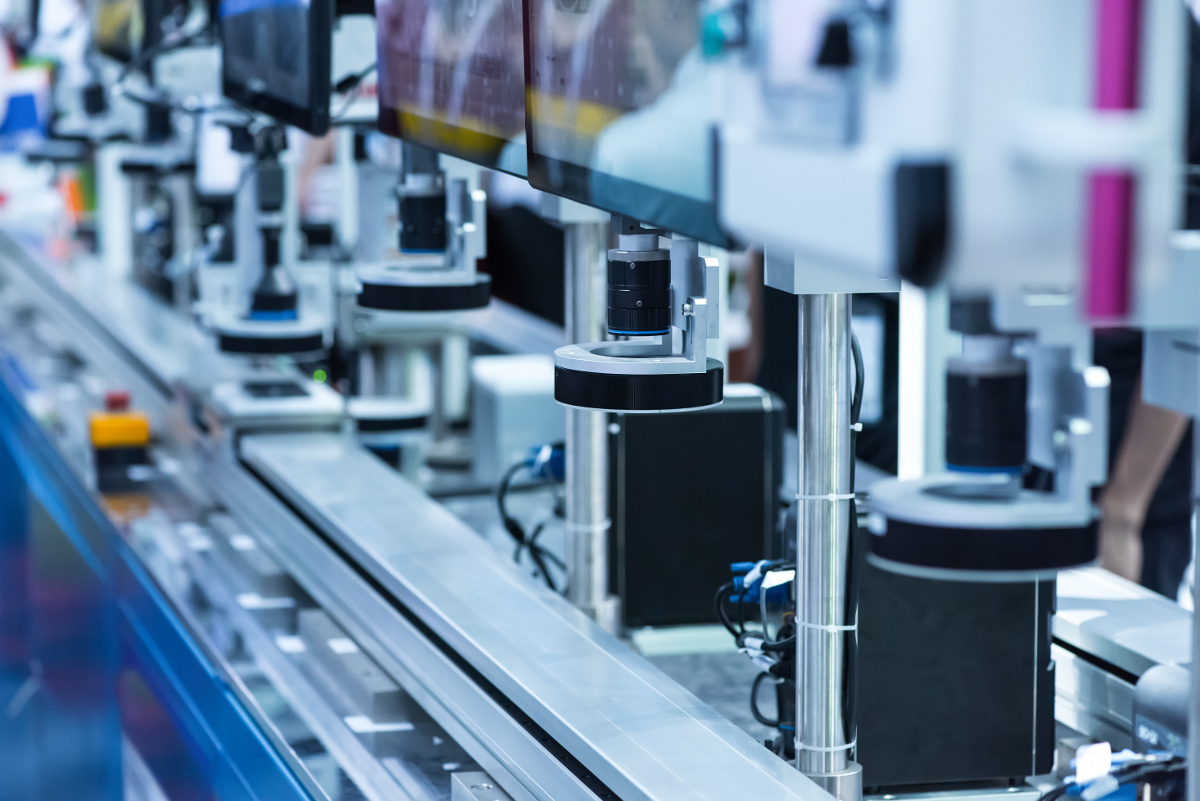
\includegraphics[width=0.8\textwidth]{industriale.jpeg}

				Automazione Industriale

				\vspace{1cm}
				
\includegraphics[width=\textwidth]{large-icon.png}

				Machine Learning
			\end{column}
		\end{columns}
	\end{frame}
	\begin{frame}{LM in Bioingegneria}
		\begin{columns}
			\begin{column}{0.4\textwidth}
				\centering
				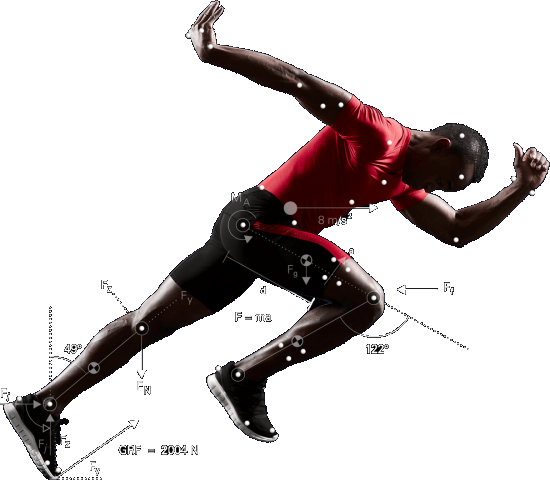
\includegraphics[width=0.7\textwidth]{Biomeccanica.png}

				Biomeccanica

				\vspace{0.5cm}
				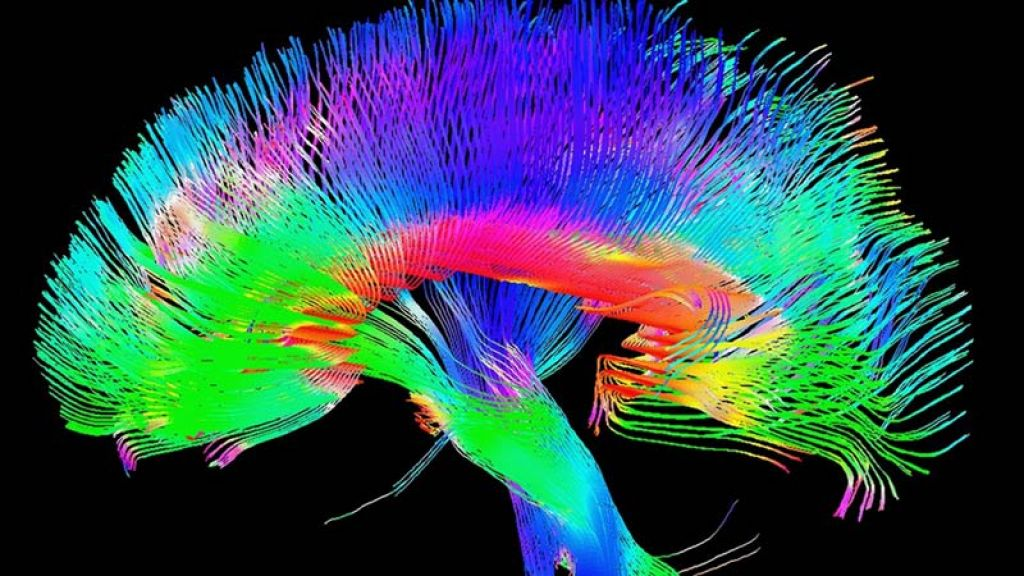
\includegraphics[width=\textwidth]{neuroimaging.jpeg}

				Neuroimaging e Segnali Biologici
			\end{column}
			\begin{column}{0.4\textwidth}
				\centering
				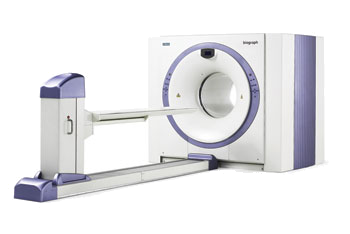
\includegraphics[width=\textwidth]{petmachine.png}

				Strumentazione Biomedica

				\vspace{1cm}
				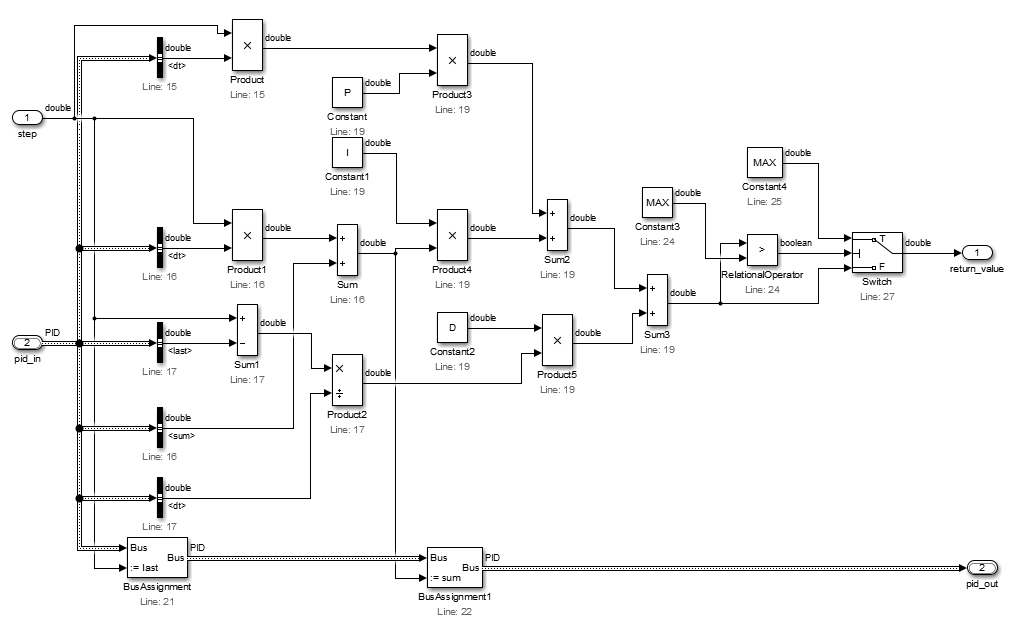
\includegraphics[width=\textwidth]{sistema_bio.png}

				Modelli e Controllo di sistemi biologici
			\end{column}
		\end{columns}
	\end{frame}
	\begin{frame}{ICT for Internet and Multimedia (ovvero Telecomunicazioni)}
		\begin{columns}
			\begin{column}{0.4\textwidth}
				\centering
				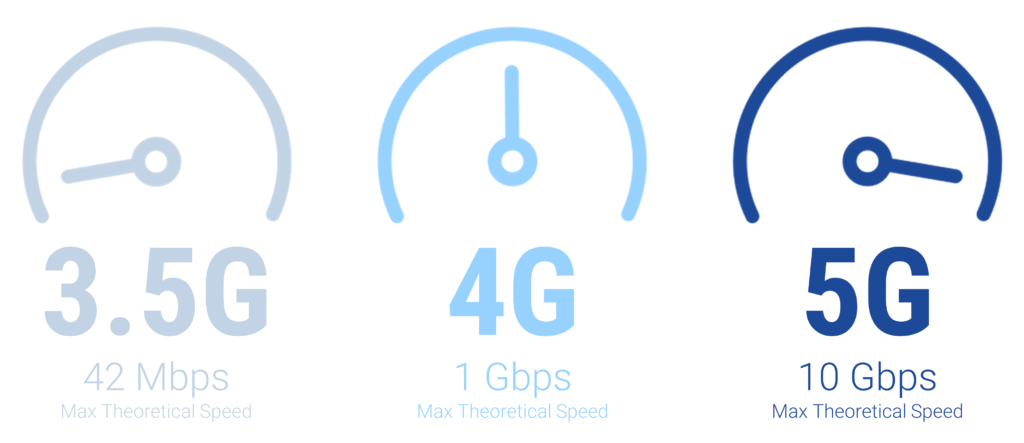
\includegraphics[width=0.6\textwidth]{5G.png}

				Progettazione delle nuove reti cellulari

				\vspace{0.4cm}
				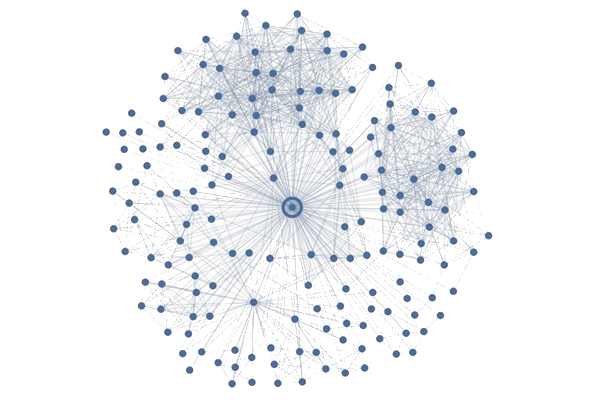
\includegraphics[width=\textwidth]{Grafo.png}

				Studio di nuovi modi per sfruttare le reti (sociali e di comunicazione)
			\end{column}
			\begin{column}{0.4\textwidth}
				\centering
				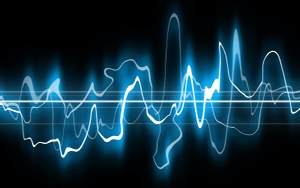
\includegraphics[width=0.6\textwidth]{signals.jpeg}

				Analisi dei segnali (visivi, biologici, acustici ecc..)

				\vspace{0.5cm}
				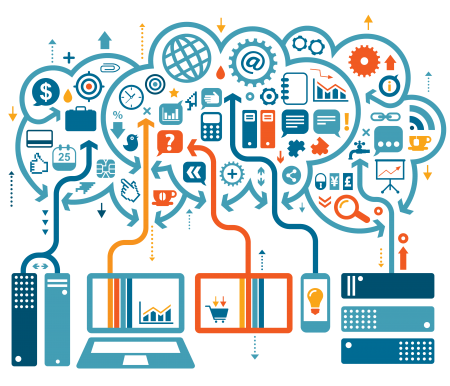
\includegraphics[width=0.6\textwidth]{big_data.png}

				Ricerca di nuovi modi per distribuire e sfruttare i dati
			\end{column}
		\end{columns}
	\end{frame}

	\begin{frame}
		\begin{description}
			\setlength\itemsep{1em}
			\item[LM in Bioingegneria] https://didattica.unipd.it/off/2018/LM/IN/IN0532
			\item[LM in Ingegneria Informatica] https://didattica.unipd.it/off/2018/LM/IN/IN0521
			\item[LM in Ingegneria Elettronica] https://didattica.unipd.it/off/2018/LM/IN/IN0520
			\item[LM in Ingegneria Automazione] https://didattica.unipd.it/off/2018/LM/IN/IN0527
			\item[ICT for Internet and Multimedia] https://didattica.unipd.it/off/2018/LM/IN/IN2371
		\end{description}
	\end{frame}


	\section{Quali sono le differenze tra triennale e magistrale?}
	\begin{frame}{Magistrale vs Triennale}
		\begin{description}
			\setlength\itemsep{1em}
			\item[Studio delle materie più attuali e di ricerca]
			\item[Maggiore progettualità]
			\item[Possibilità di fare delle pubblicazioni]
		\end{description}
	\end{frame}
	\begin{frame}
		\centering
		\begin{figure}
	  		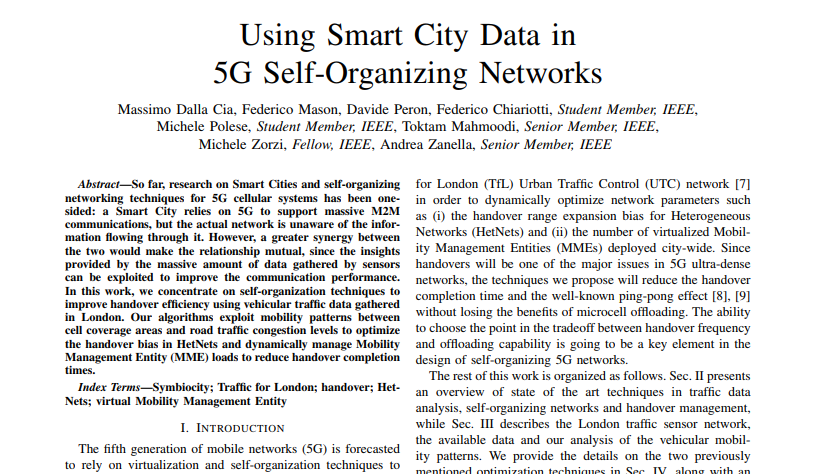
\includegraphics[width=10cm]{articolo.png}
	  	\end{figure}
	\end{frame}


	\section{E se voglio studiare all'estero?}
	\begin{frame}{Erasmus+}
		\centering
		\begin{figure}
	  		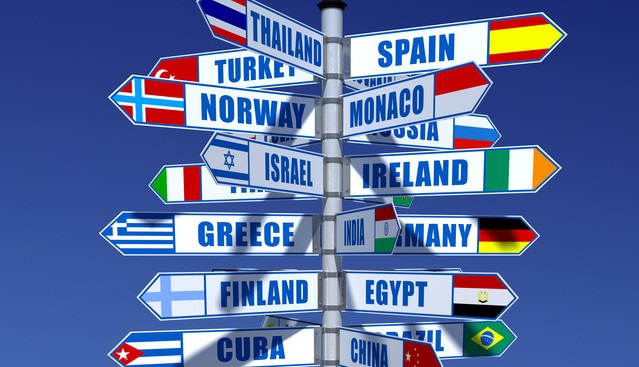
\includegraphics[width=10cm]{Erasmus.jpg}
	  	\end{figure}
	\end{frame}

\end{document}